В ходе выполнения данного этапа я последовательно определял максимально допустимые уровни шумов, рассинхронизации и граничного напряжения, при которых сохраняется качественная передача сообщения.

Сначала я изменял уровень шумов \textbf{Noise} и определял его максимально допустимое значение при нулевых значениях остальных параметров.

Затем устанавливал уровень шумов в ноль и изменял уровень рассинхронизации \textbf{Desync}. Находил его максимально допустимое значение, при котором сообщение передается без ошибок.

Затем при нулевых значениях шумов и рассинхронизации я изменял уровень граничного напряжения \textbf{Voltage} и определял его максимально допустимое значение.


\subsection{NRZ}

\subsubsection{Noise}

Максимально допустимый уровень шума был определён с помощью программы \textit{Network Fourier} и составил \textbf{0.2}. Это граничное значение, при котором сигнал не искажается при воздействии произвольных гармоник.

\vspace{0.4cm}
\begin{figure}[h]
	\centering
	% 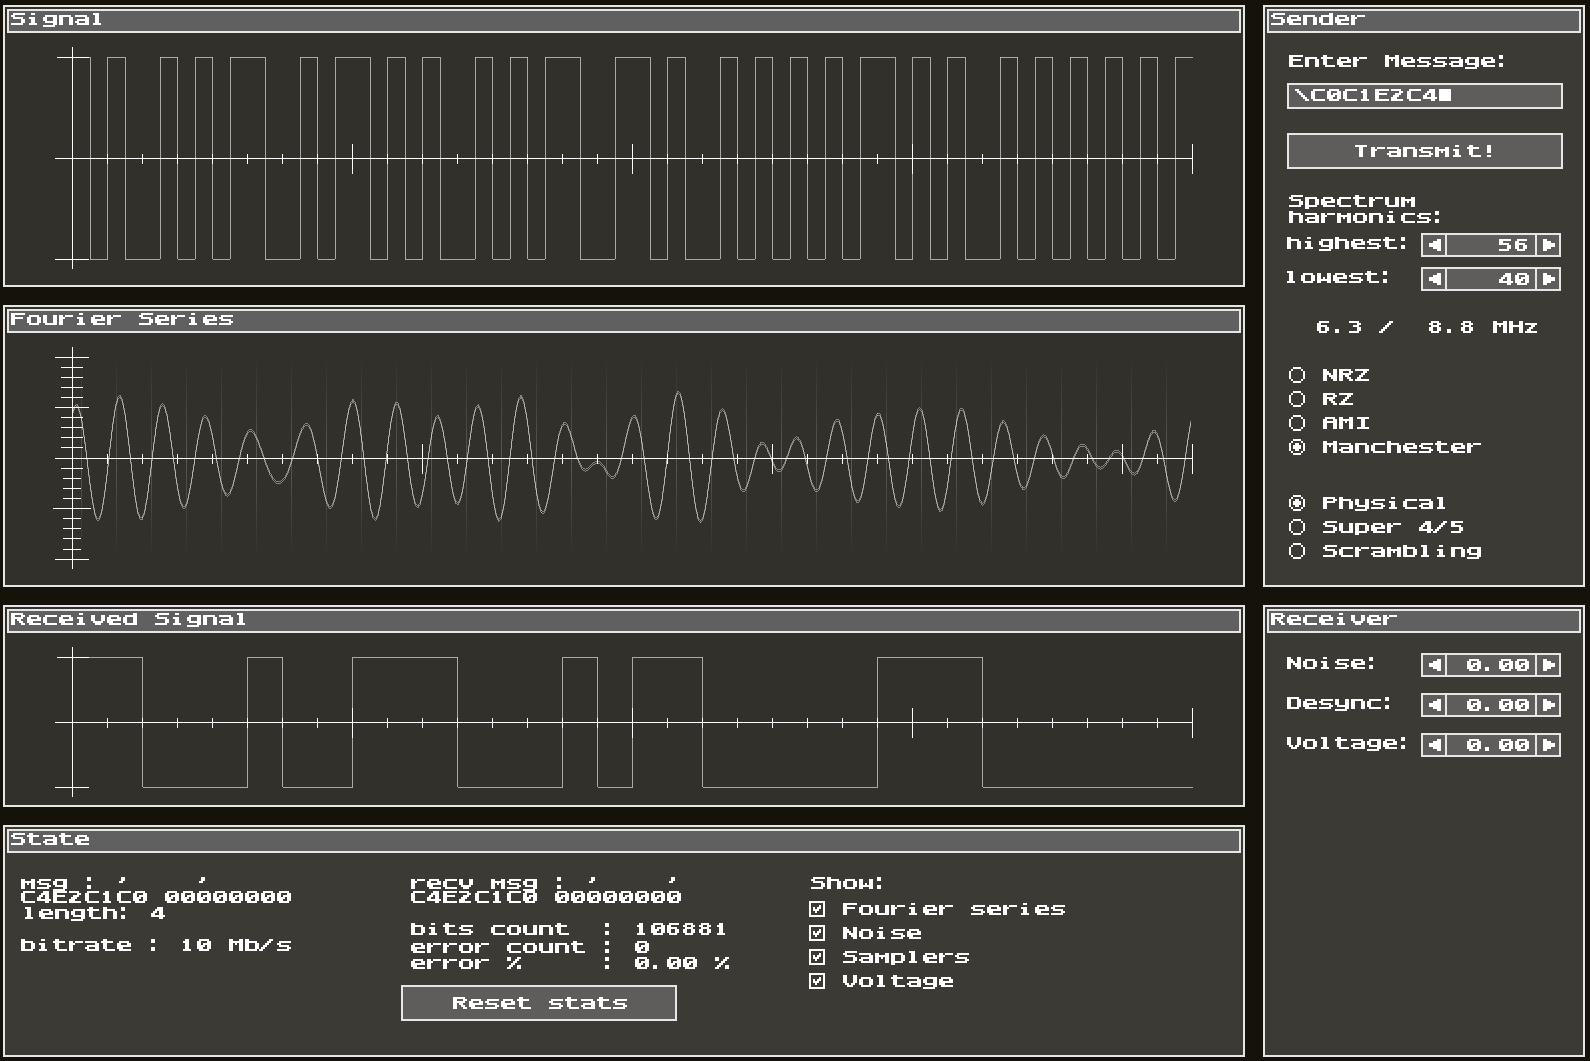
\includegraphics[width=0.95\linewidth]{./data/ideal_m2_min_f.png}
	\cutpic{0.2cm}{17cm}{./data/noise_nrz.png}
	\caption{Максимально допустимый уровень шума 0.2 для NRZ}
\end{figure}

\subsubsection{Desync}

Максимально допустимый уровень рассинхронизации был определён с помощью программы \textit{Network Fourier} и составил \textbf{0.35}. Это граничное значение, при котором различие часов передатчика и приёмника не искажают сигнал.

\vspace{0.4cm}
\begin{figure}[h]
	\centering
	% 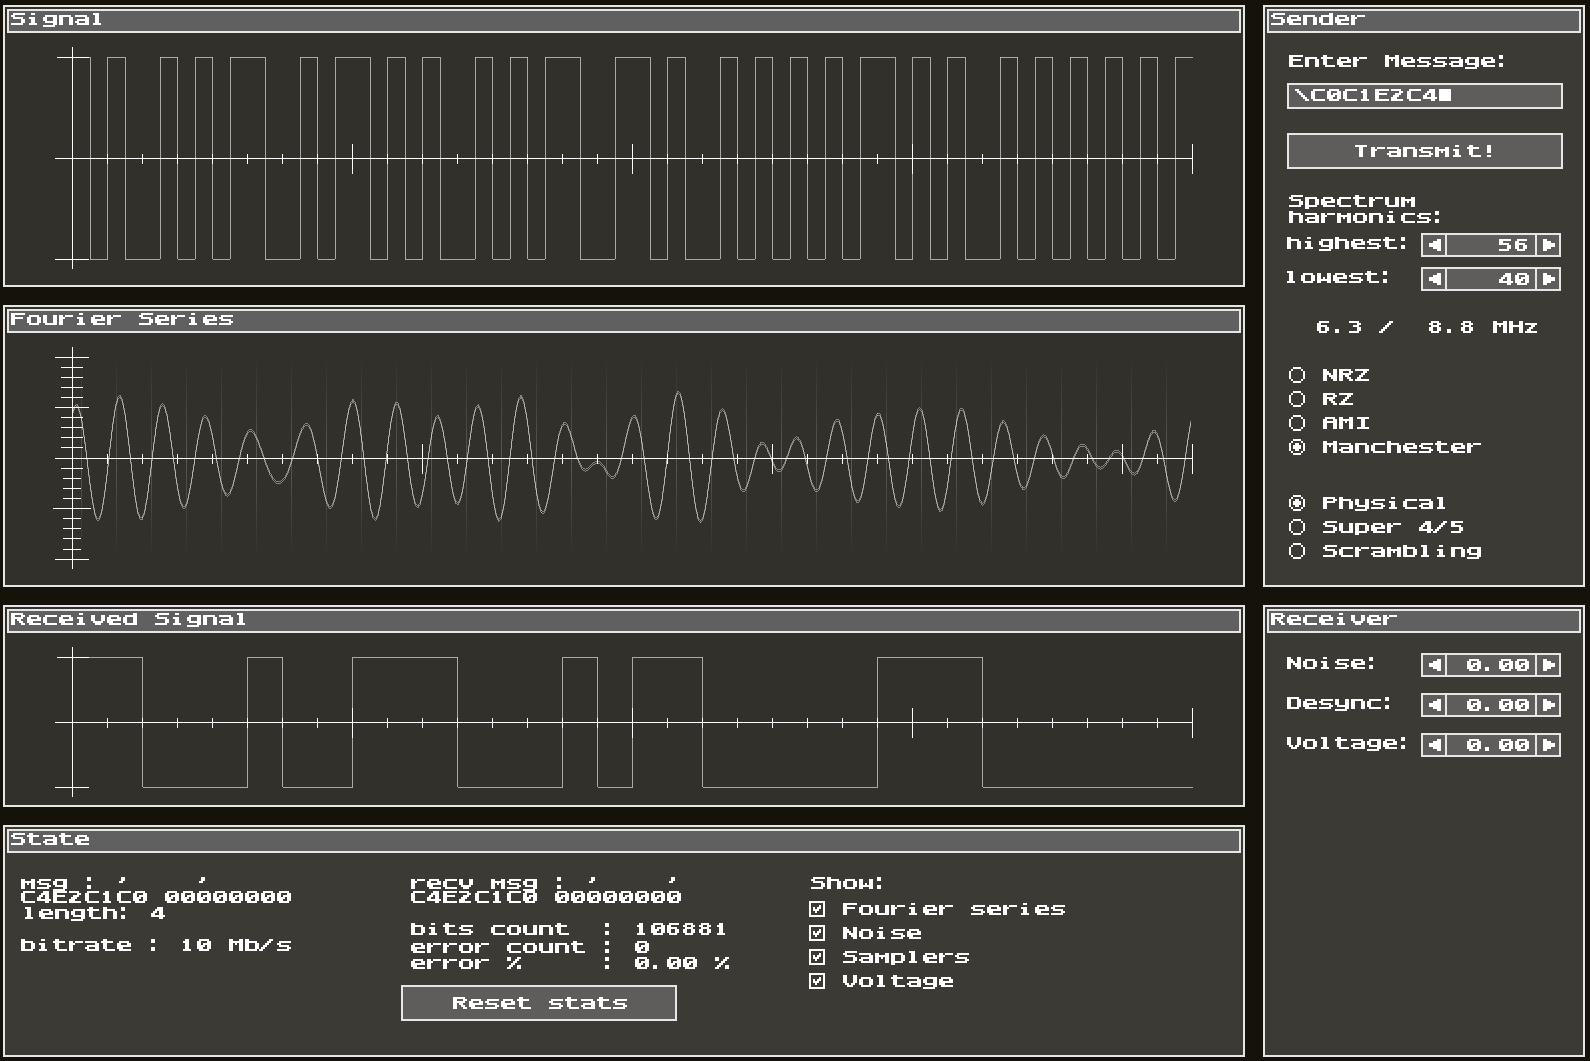
\includegraphics[width=0.95\linewidth]{./data/ideal_m2_min_f.png}
	\cutpic{0.2cm}{17cm}{./data/desync_nrz.png}
	\caption{Максимально допустимый уровень рассинхрона 0.35 для NRZ}
\end{figure}

\subsubsection{Voltage}

\begin{wrapfigure}{l}{0.7\textwidth}
	\centering
	% 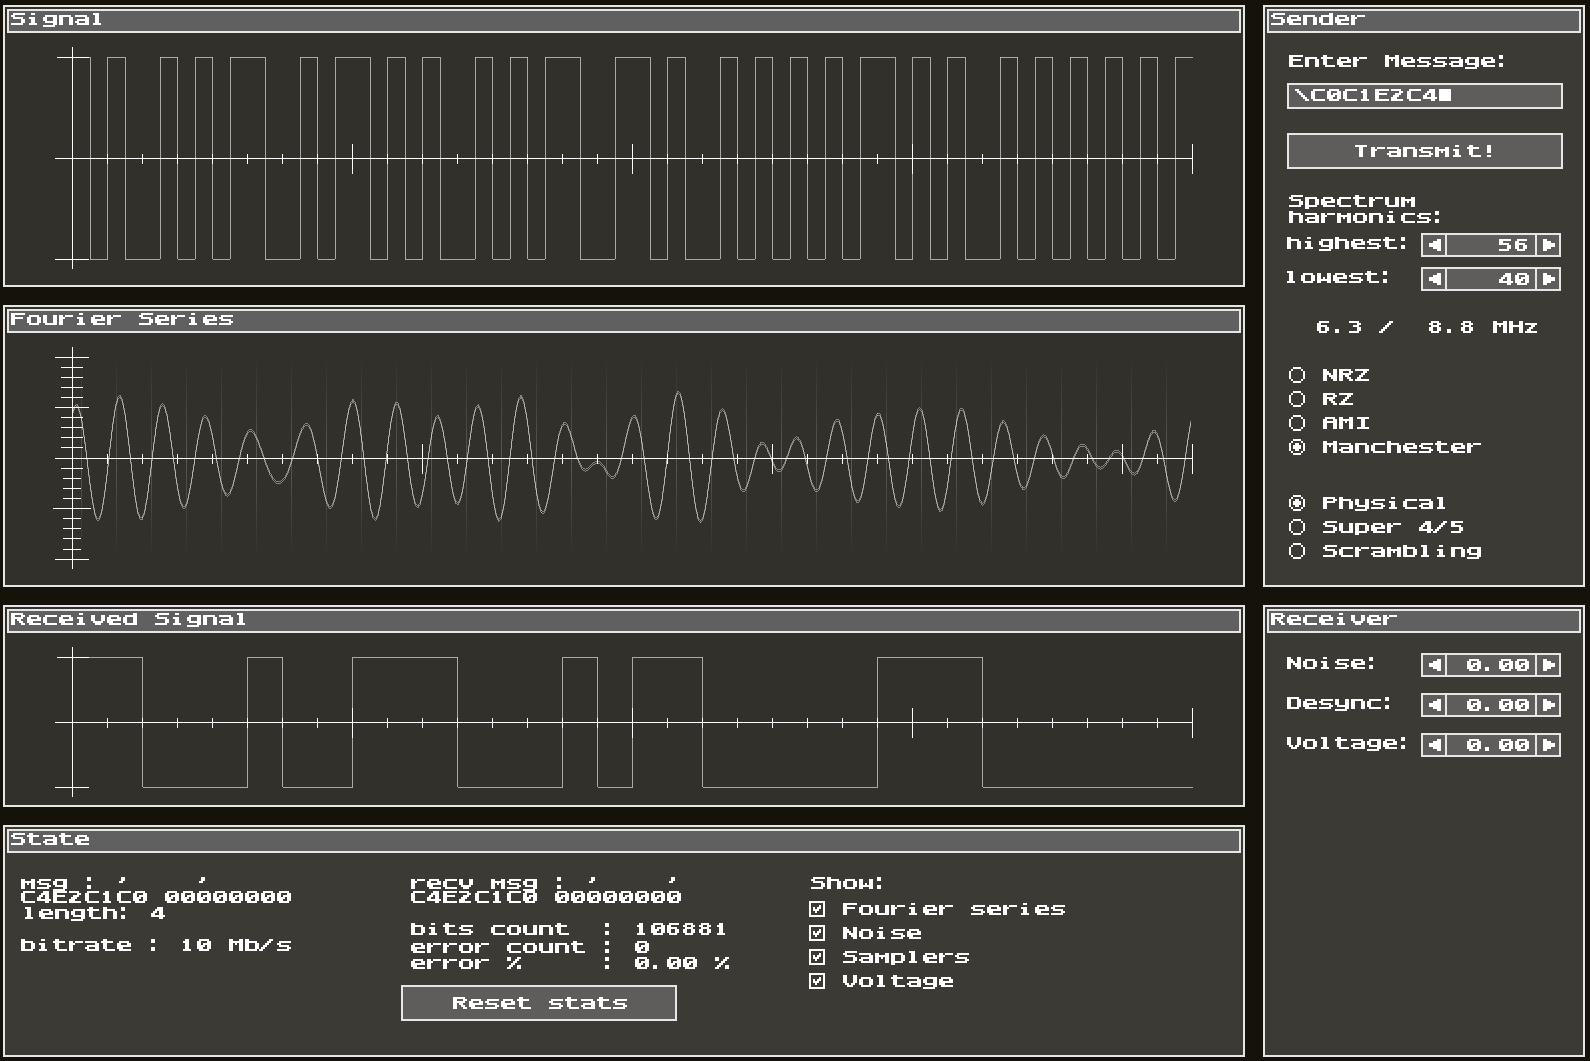
\includegraphics[width=0.95\linewidth]{./data/ideal_m2_min_f.png}
	\cutpic{0.2cm}{12cm}{./data/voltage_nrz.png}
	\caption{Уровень напряжения 0.38 для NRZ}
	\vspace{-100pt}
\end{wrapfigure}

Максимально допустимый уровень напряжения был определён с помощью программы \textit{Network Fourier} и составил \textbf{0.38}. Это граничное значение, ниже которого мы не будем считывать сигнал.


% ------------------------------------------------


\subsection{RZ}

\subsubsection{Noise}

Максимально допустимый уровень шума был определён с помощью программы \textit{Network Fourier} и составил \textbf{0.02}. Это граничное значение, при котором сигнал не искажается при воздействии произвольных гармоник.

\vspace{0.4cm}
\begin{figure}[h]
	\centering
	% 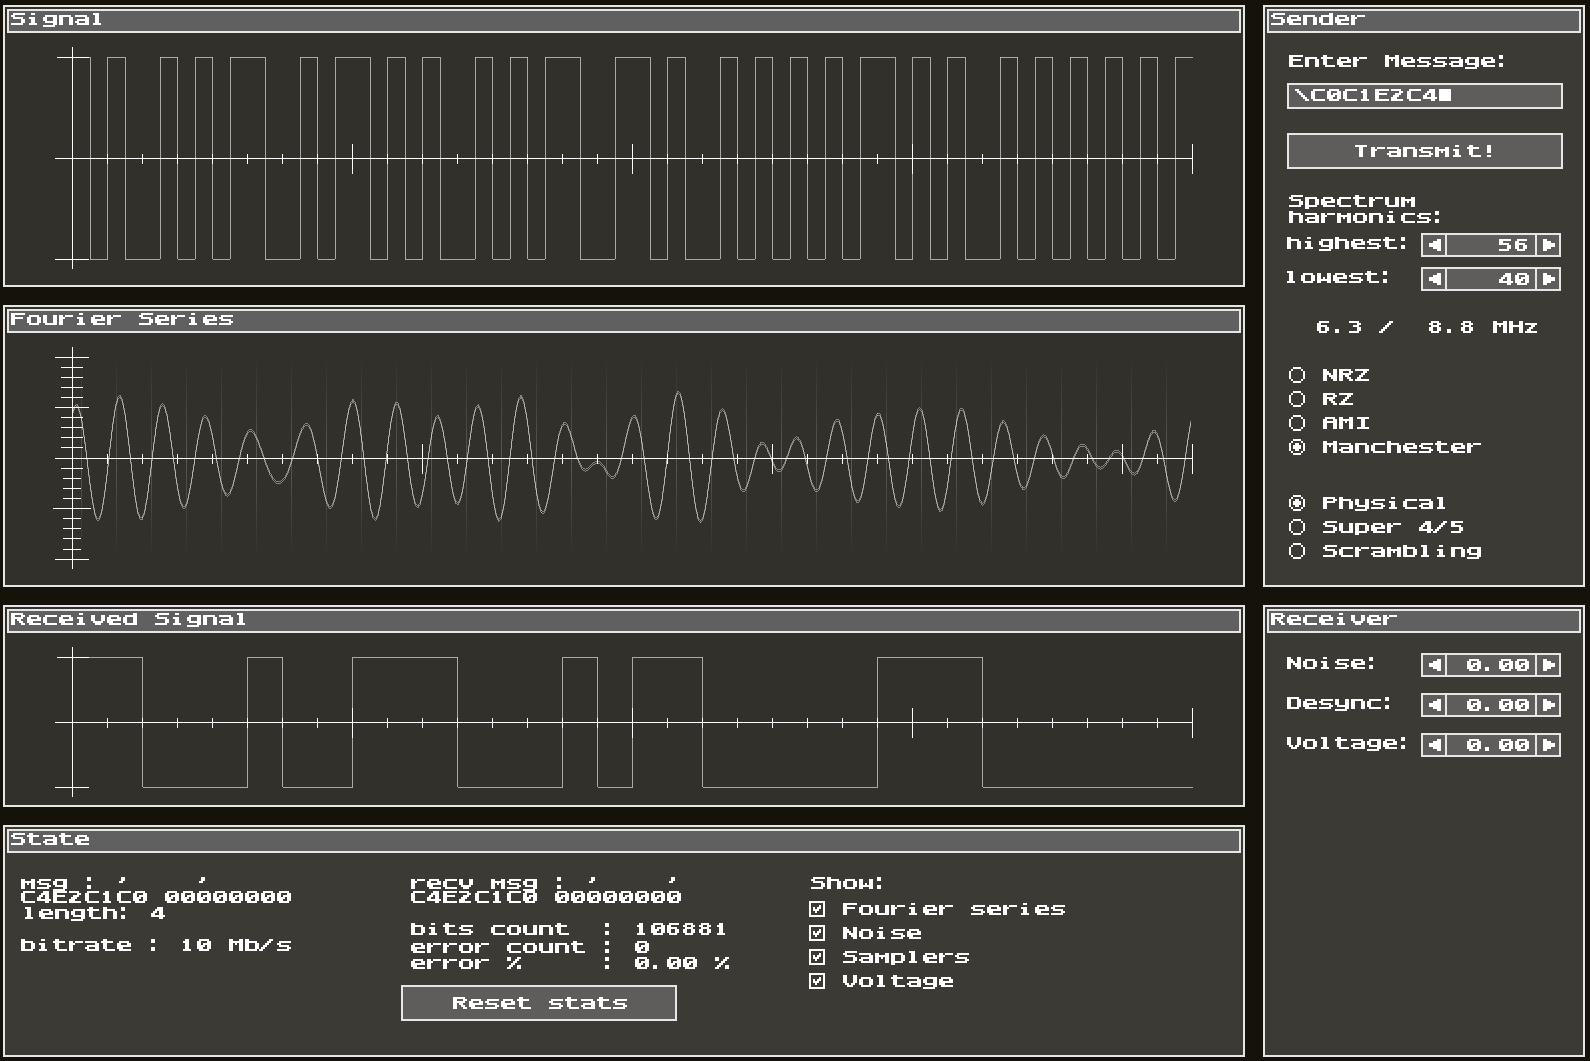
\includegraphics[width=0.95\linewidth]{./data/ideal_m2_min_f.png}
	\cutpic{0.2cm}{17cm}{./data/noise_rz.png}
	\caption{Максимально допустимый уровень шума 0.02 для RZ}
\end{figure}

\subsubsection{Desync}

\vspace{-0.2cm}
\begin{wrapfigure}{r}{0.65\textwidth}
	\centering
	% 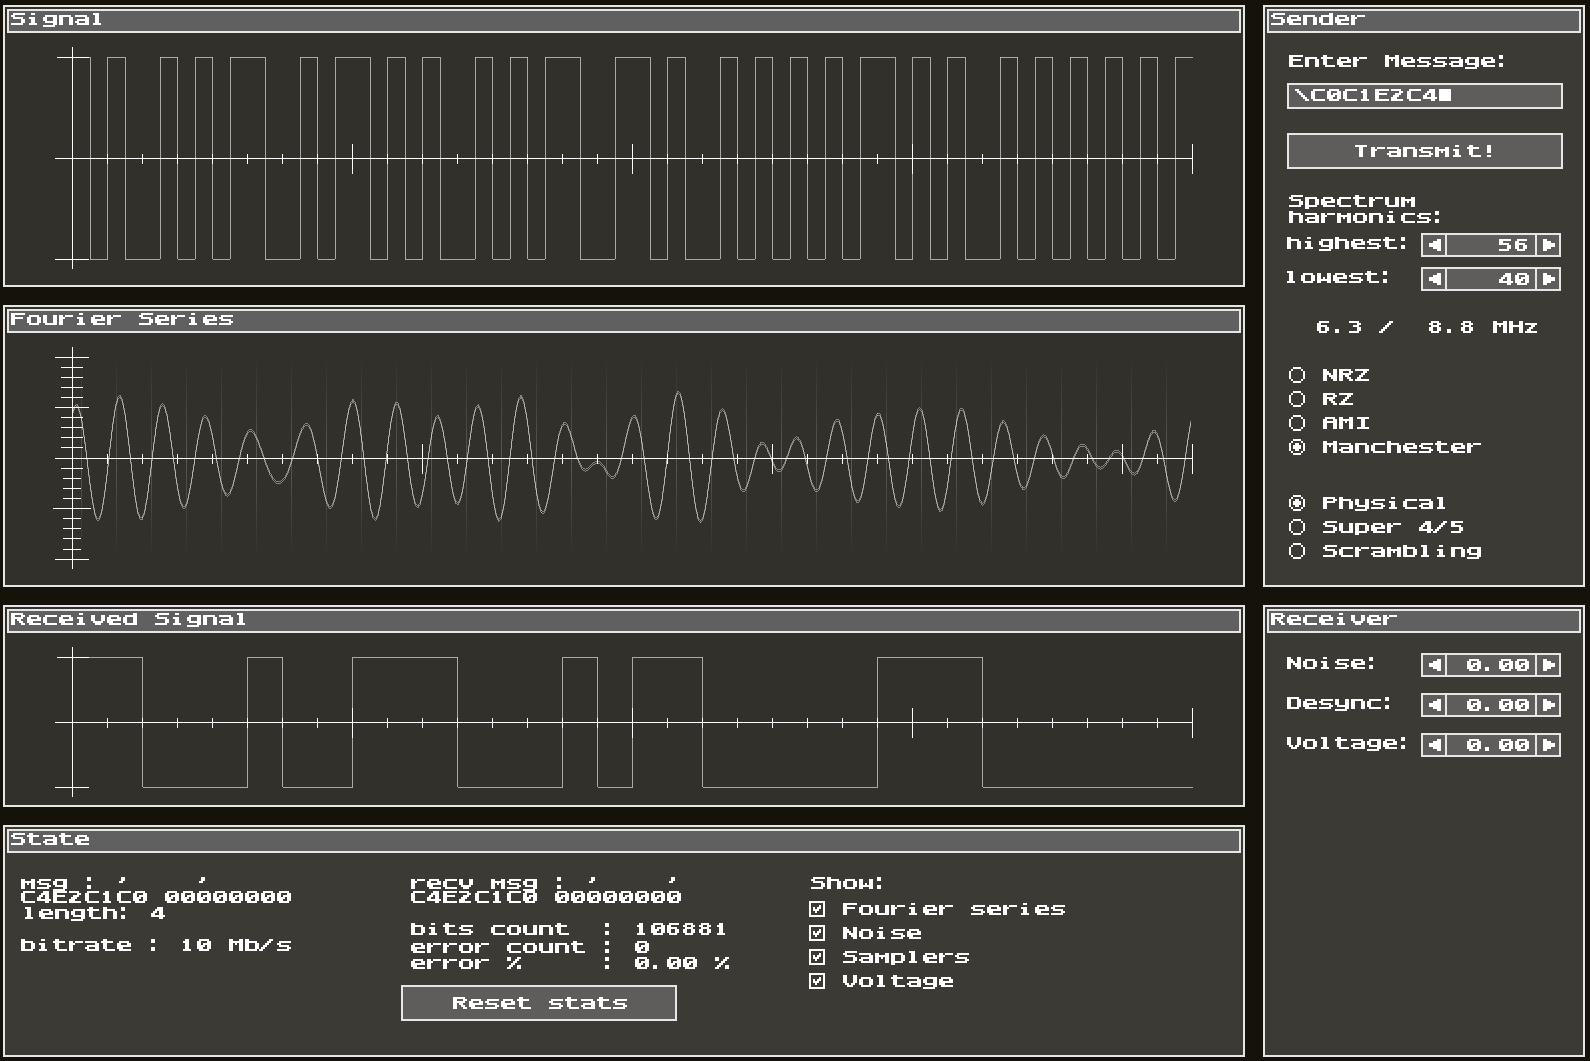
\includegraphics[width=0.95\linewidth]{./data/ideal_m2_min_f.png}
	\cutpic{0.2cm}{11.5cm}{./data/3_rz_desync.png.jpg}
	\caption{Уровень рассинхрона 0.02 для RZ}
	\vspace{-125pt}
\end{wrapfigure}

Максимально допустимый уровень рассинхронизации был определён с помощью программы \textit{Network Fourier} и составил \textbf{0.02}. Это граничное значение, при котором различие часов передатчика и приёмника не искажают сигнал.
\thispagestyle{empty}

\newpage

\subsubsection{Voltage}
Максимально допустимый уровень напряжения был определён с помощью программы \textit{Network Fourier} и составил \textbf{0.16}. Это граничное значение, ниже которого мы не будем считывать сигнал.

\vspace{0.4cm}
\begin{figure}[h]
	\centering
	% 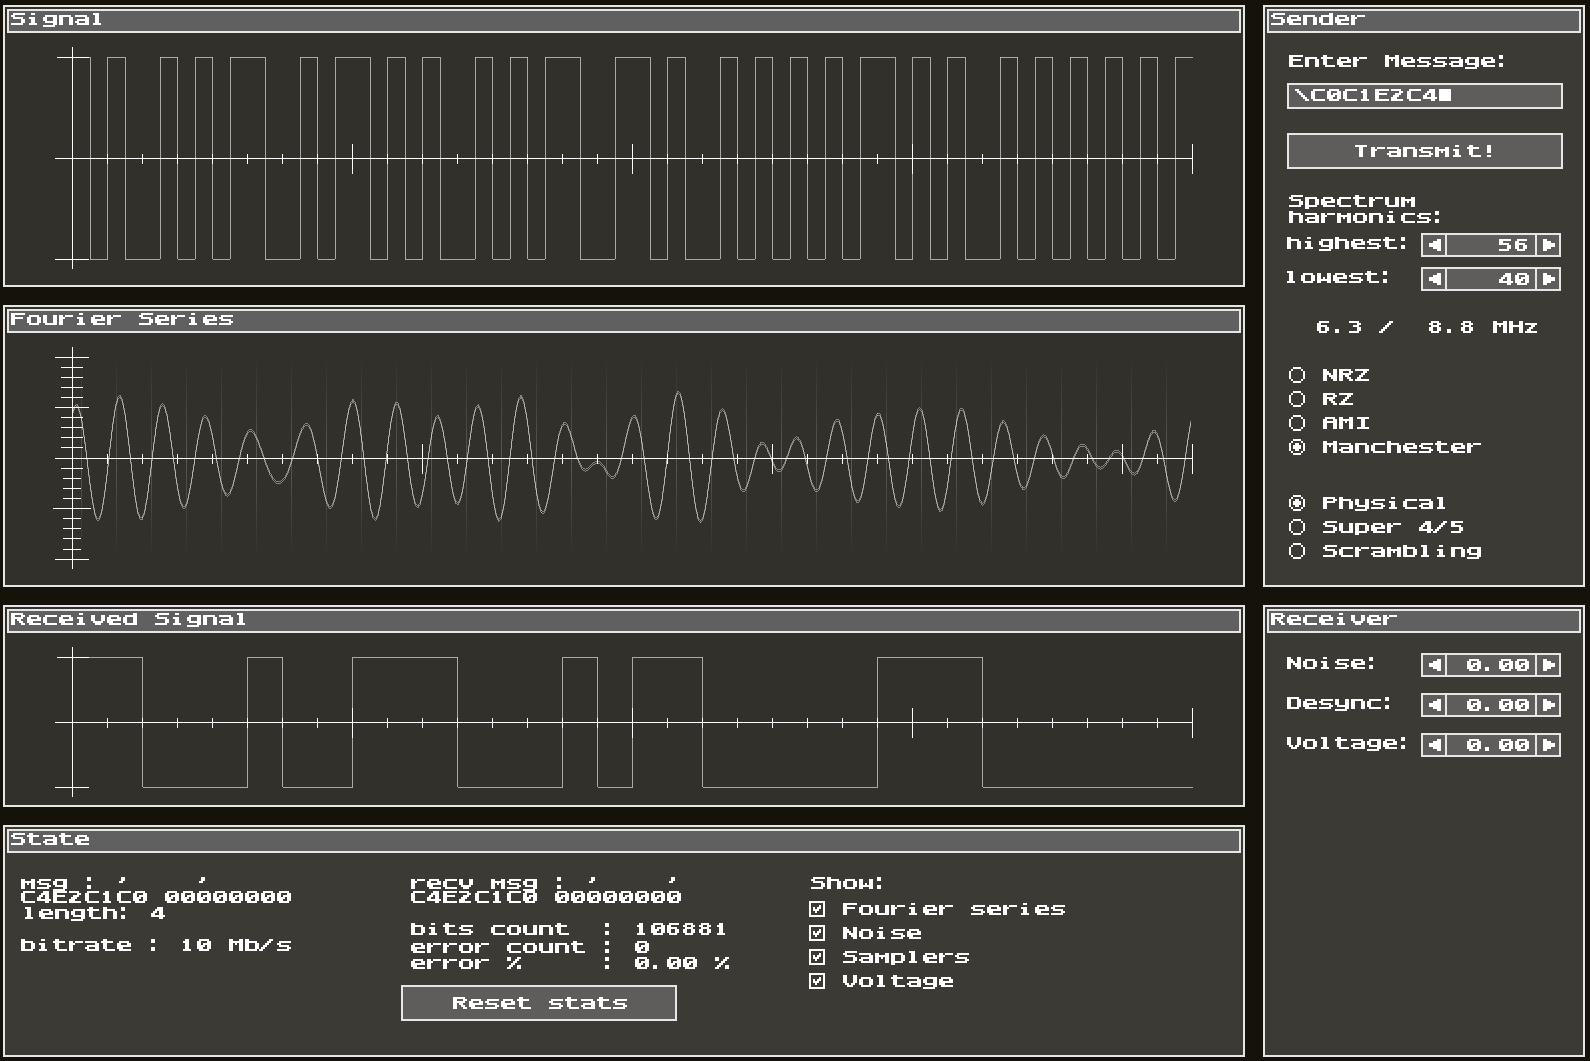
\includegraphics[width=0.95\linewidth]{./data/ideal_m2_min_f.png}
	\cutpic{0.2cm}{15cm}{./data/3_rz_voltage.png.jpg}
	\caption{Максимально допустимый уровень напряжения 0.16 для RZ}
\end{figure}


% ------------------------------------------------


\subsection{M2}

\subsubsection{Noise}

\vspace{-0.2cm}
\begin{wrapfigure}{r}{0.65\textwidth}
    \centering
    \cutpic{0.2cm}{11.5cm}{./data/3_m2_noise.png.jpg}
    \caption{Уровень шума 0.16 для M2}
    \vspace{-5cm}
\end{wrapfigure}
\thispagestyle{empty}

Максимально допустимый уровень шума был определён с помощью программы \textit{Network Fourier} и составил \textbf{0.16}. Это граничное значение, при котором сигнал не искажается при воздействии произвольных гармоник.

\newpage

\subsubsection{Desync}

Максимально допустимый уровень рассинхронизации был определён с помощью программы \textit{Network Fourier} и составил \textbf{0.1}. Это граничное значение, при котором различие часов передатчика и приёмника не искажают сигнал.

\vspace{0.4cm}
\begin{figure}[h]
	\centering
	% 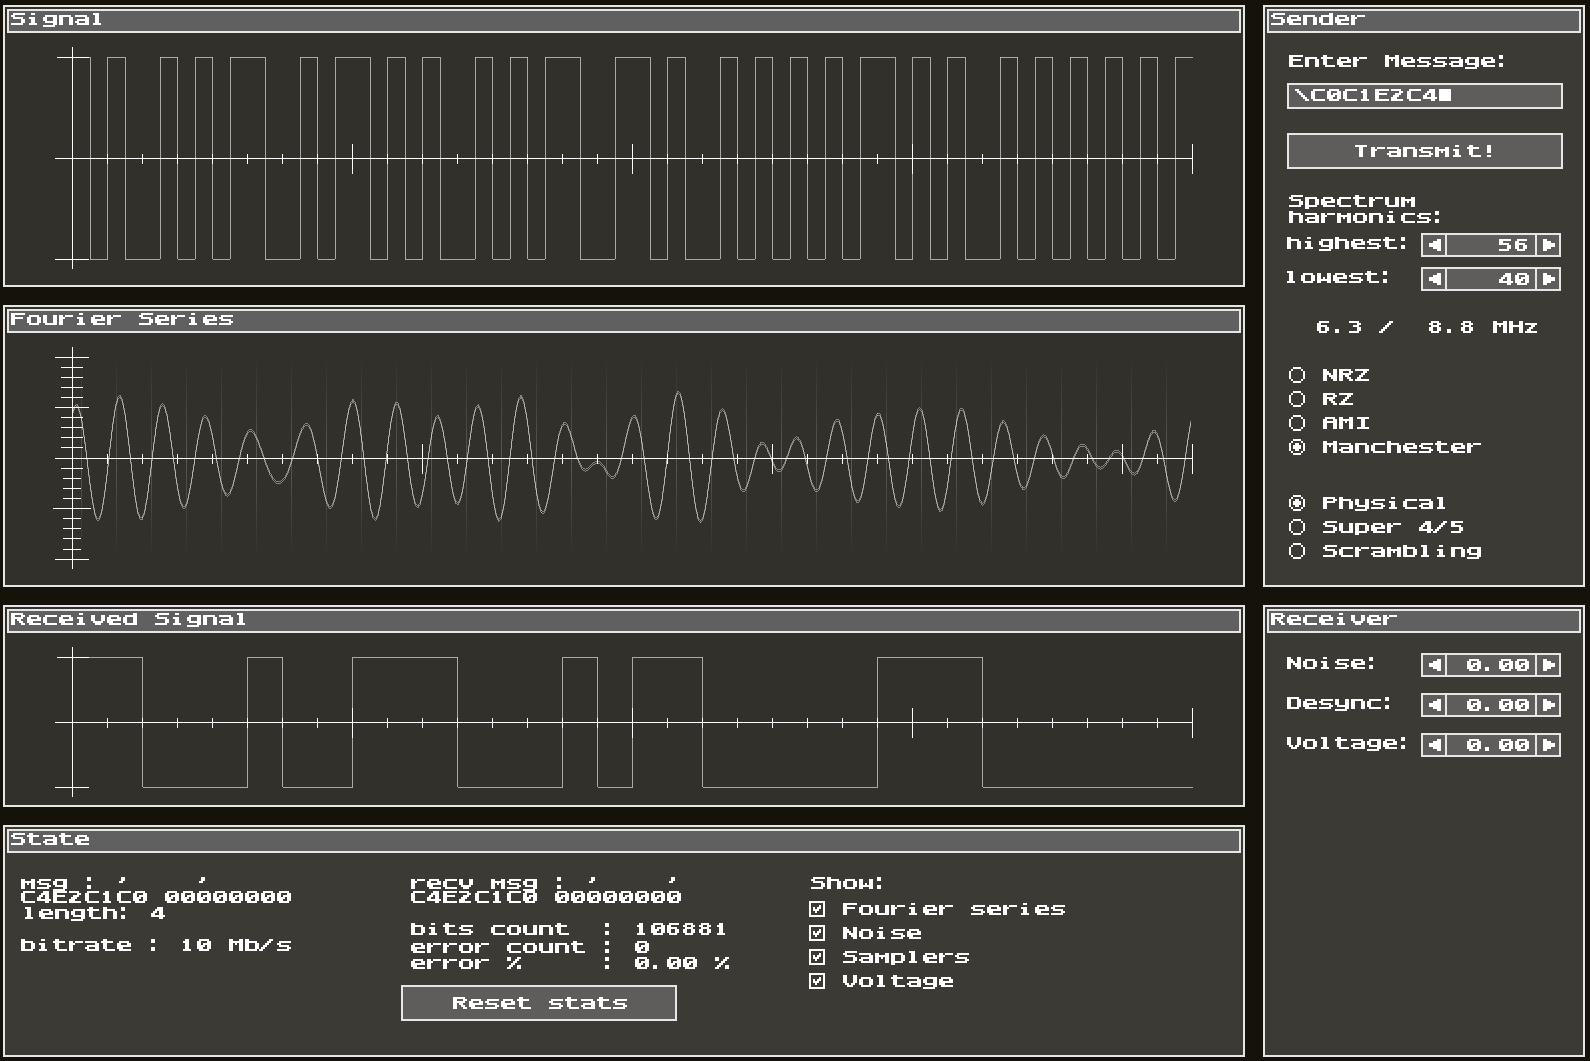
\includegraphics[width=0.95\linewidth]{./data/ideal_m2_min_f.png}
	\cutpic{0.2cm}{11.2cm}{./data/3_m2_desync.png.jpg}
	\caption{Максимально допустимый уровень рассинхронизации 0.1 для M2}
\end{figure}

\subsubsection{Voltage}

Максимально допустимый уровень напряжения был определён с помощью программы \textit{Network Fourier} и составил \textbf{0.1}. Это граничное значение, ниже которого мы не будем считывать сигнал.

\vspace{0.4cm}
\begin{figure}[h]
	\centering
	% 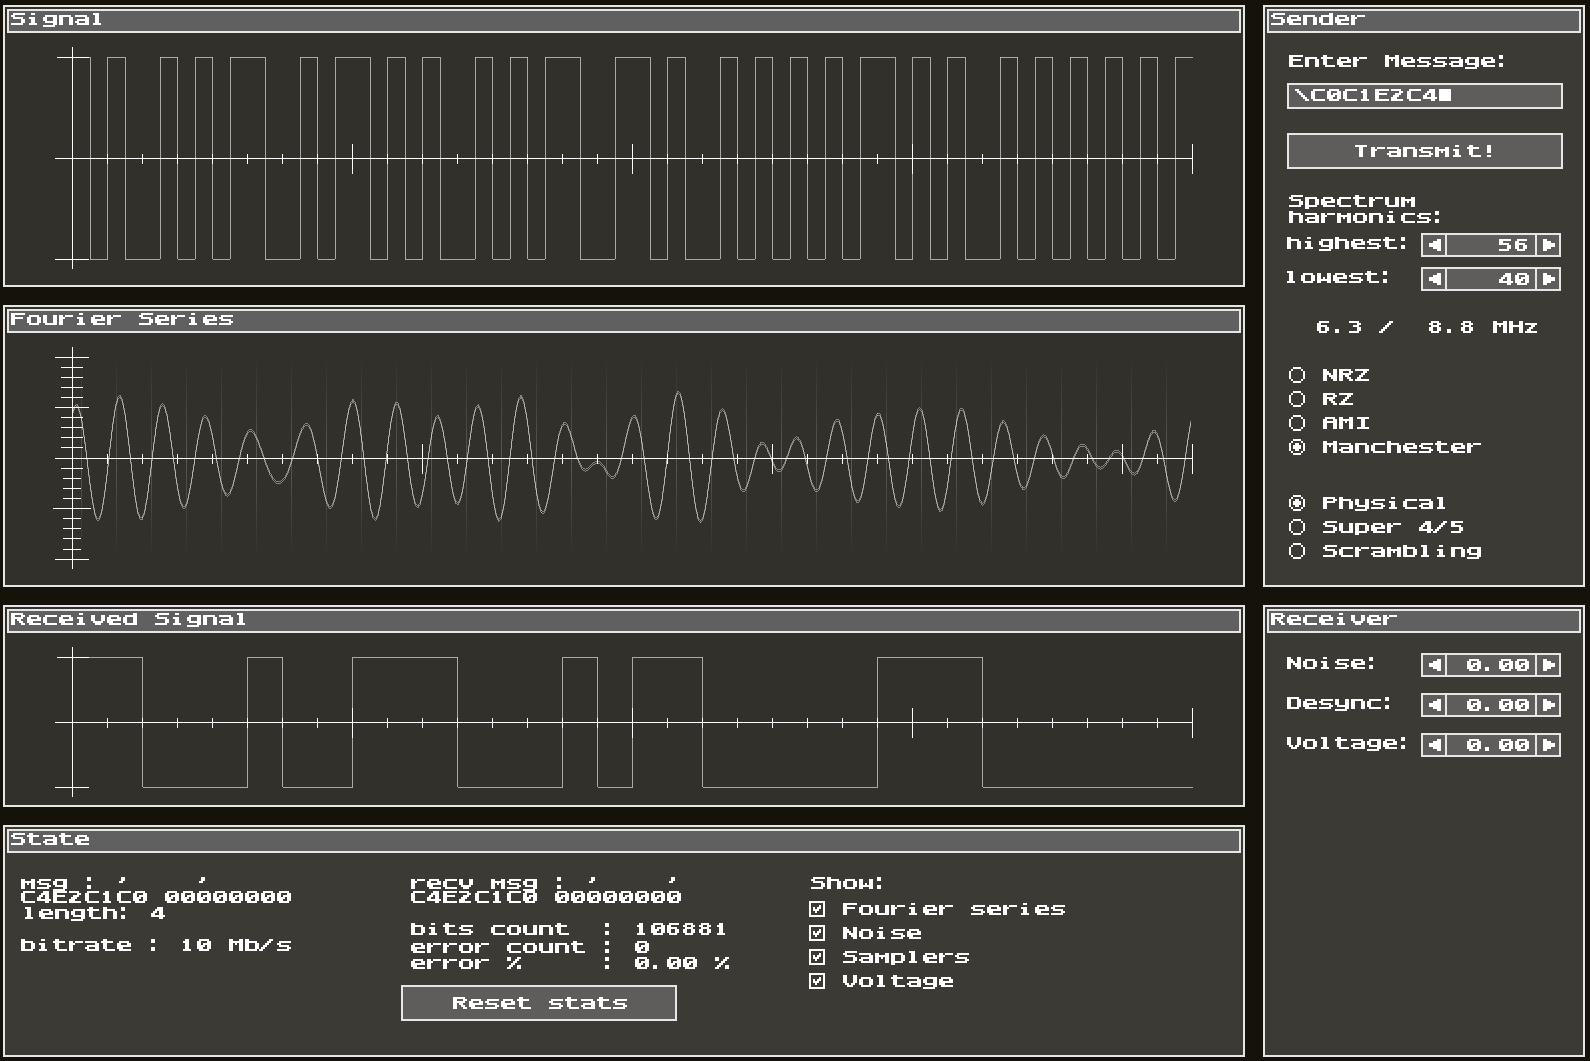
\includegraphics[width=0.95\linewidth]{./data/ideal_m2_min_f.png}
	\cutpic{0.2cm}{11.5cm}{./data/3_m2_voltage.png.jpg}
	\caption{Максимально допустимый уровень напряжения 1 для M2}
\end{figure}


% ------------------------------------------------


\newpage
\subsection{NRZ + 4B/5B}

\subsubsection{Noise}

Максимально допустимый уровень шума был определён с помощью программы \textit{Network Fourier} и составил \textbf{0.02}. Это граничное значение, при котором сигнал не искажается при воздействии произвольных гармоник.

\vspace{0.4cm}
\begin{figure}[h]
	\centering
	% 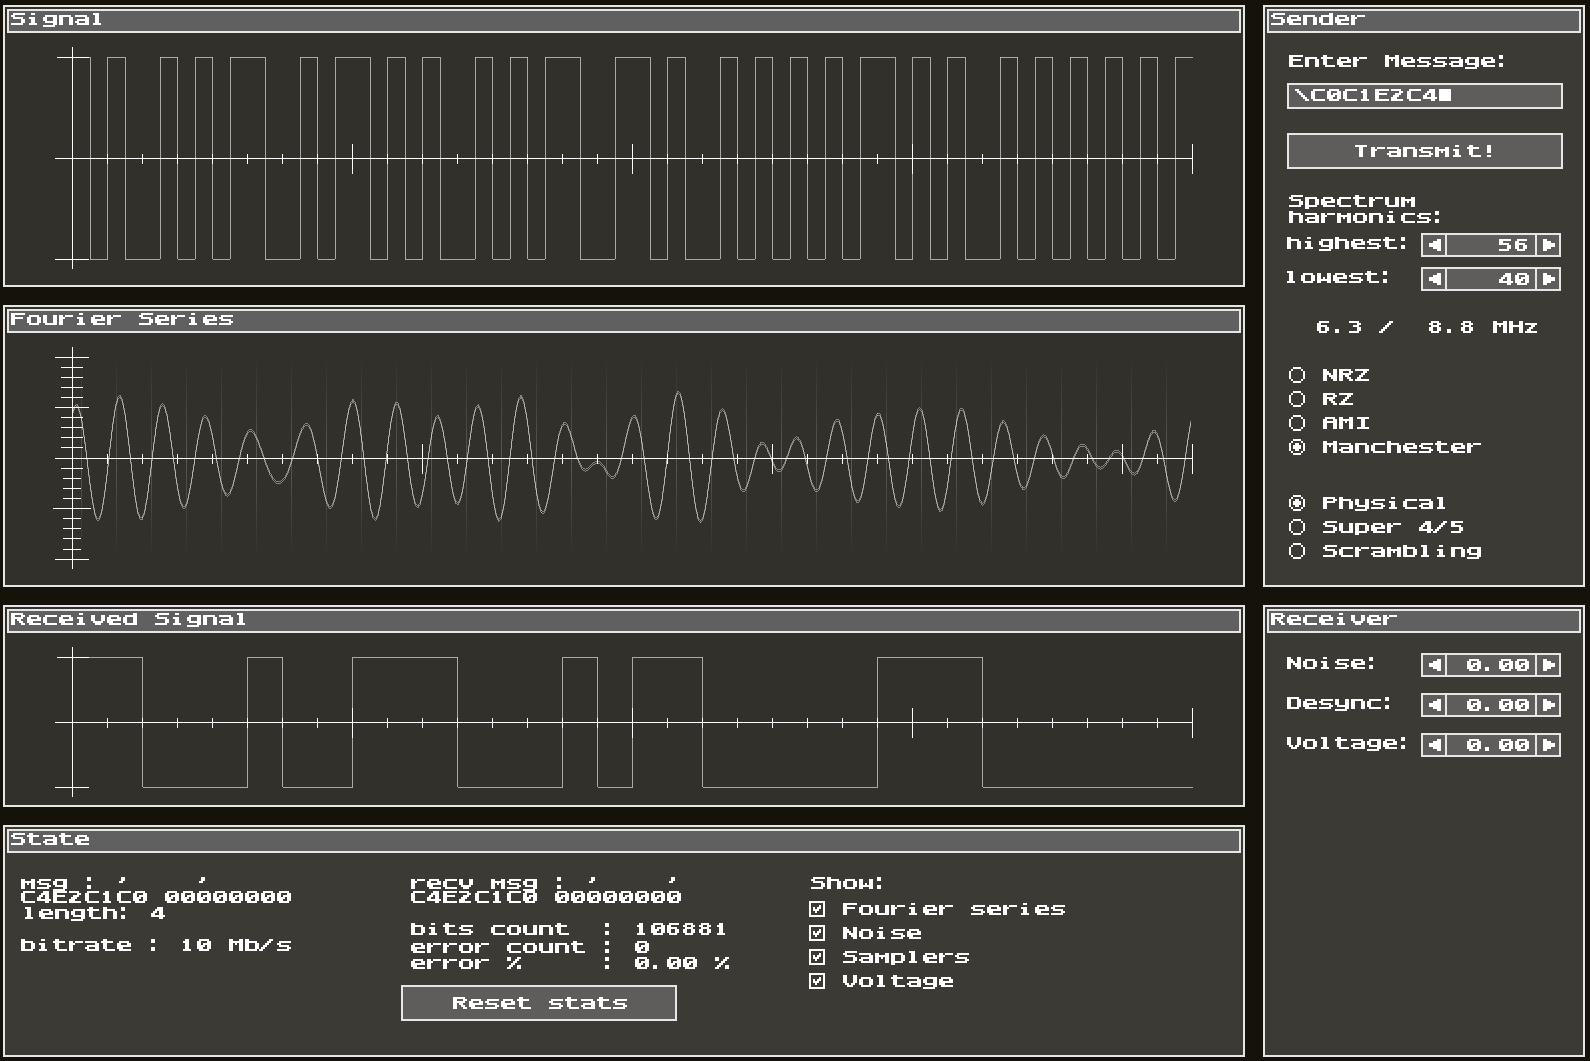
\includegraphics[width=0.95\linewidth]{./data/ideal_m2_min_f.png}
	\cutpic{0.2cm}{15cm}{./data/3_nrz45_noise.png.jpg}
	\caption{Максимально допустимый уровень шума 0.02 для NRZ+4B/5B}
\end{figure}

\subsubsection{Desync}

\vspace{-0.2cm}
\begin{wrapfigure}{r}{0.65\textwidth}
	\centering
	% 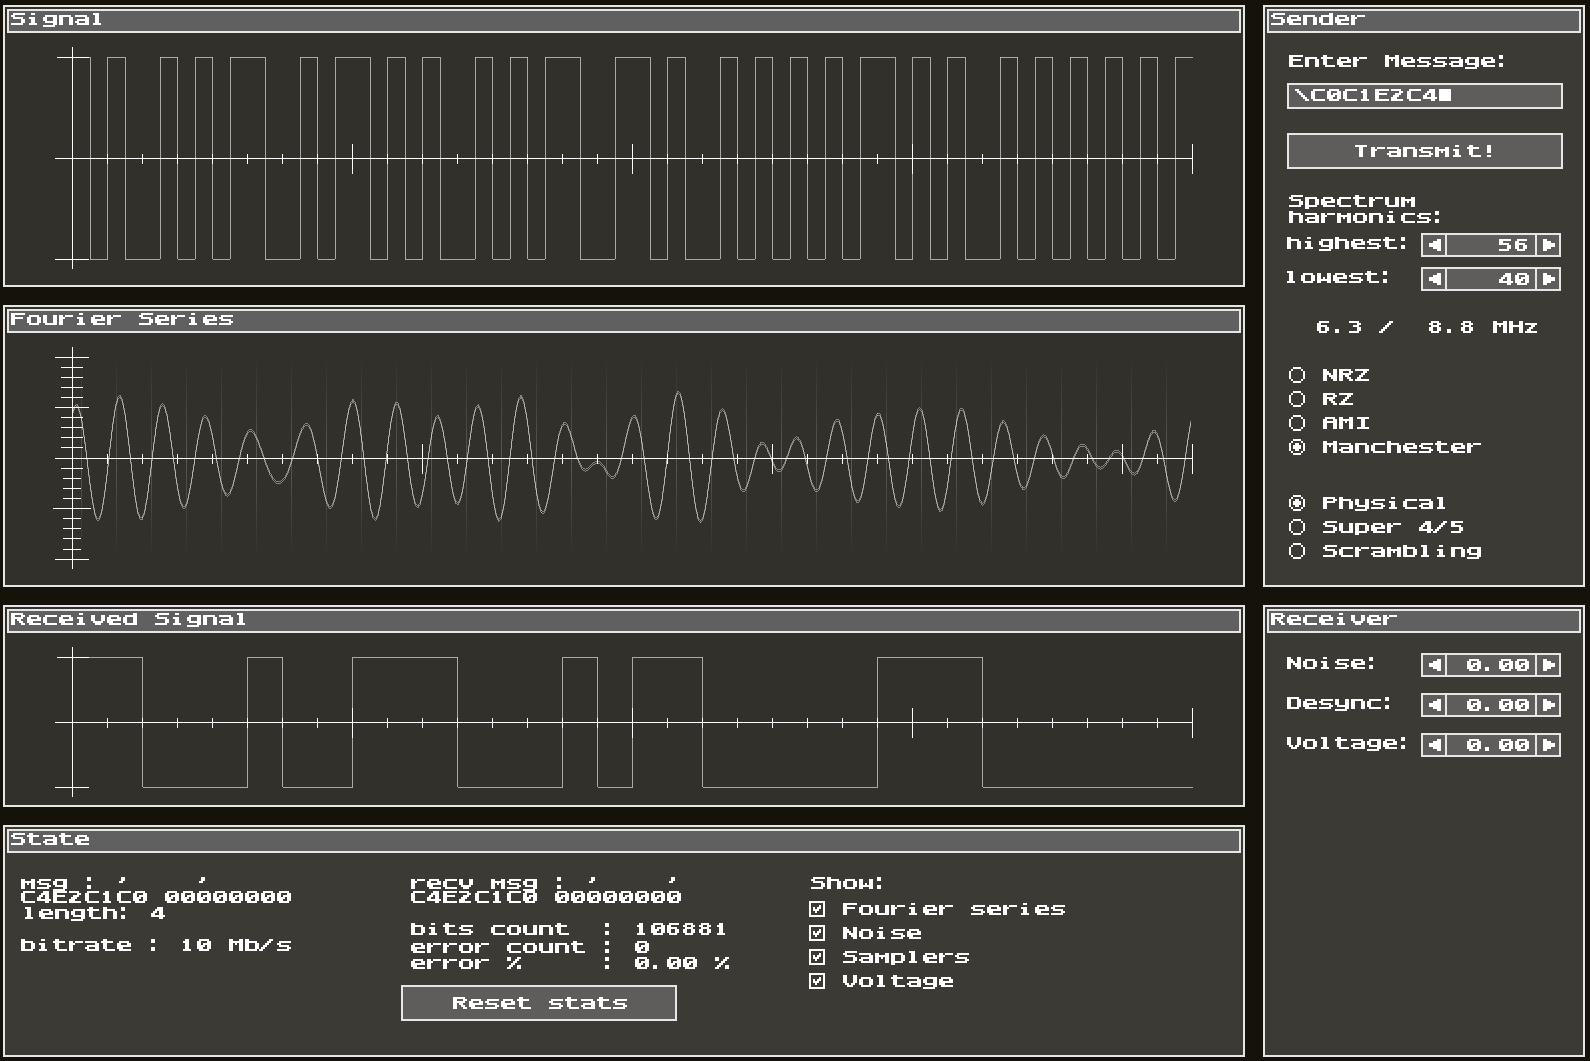
\includegraphics[width=0.95\linewidth]{./data/ideal_m2_min_f.png}
	\cutpic{0.2cm}{11.5cm}{./data/3_nrz45_desync.png.jpg}
	\caption{Уровень рассинхрона 0.12 для NRZ+4B/5B}
	\vspace{-125pt}
\end{wrapfigure}

Максимально допустимый уровень рассинхронизации был определён с помощью программы \textit{Network Fourier} и составил \textbf{0.12}. Это граничное значение, при котором различие часов передатчика и приёмника не искажают сигнал.
\thispagestyle{empty}

\newpage

\subsubsection{Voltage}
Максимально допустимый уровень напряжения был определён с помощью программы \textit{Network Fourier} и составил \textbf{0.02}. Это граничное значение, ниже которого мы не будем считывать сигнал.

\vspace{0.4cm}
\begin{figure}[h]
	\centering
	% 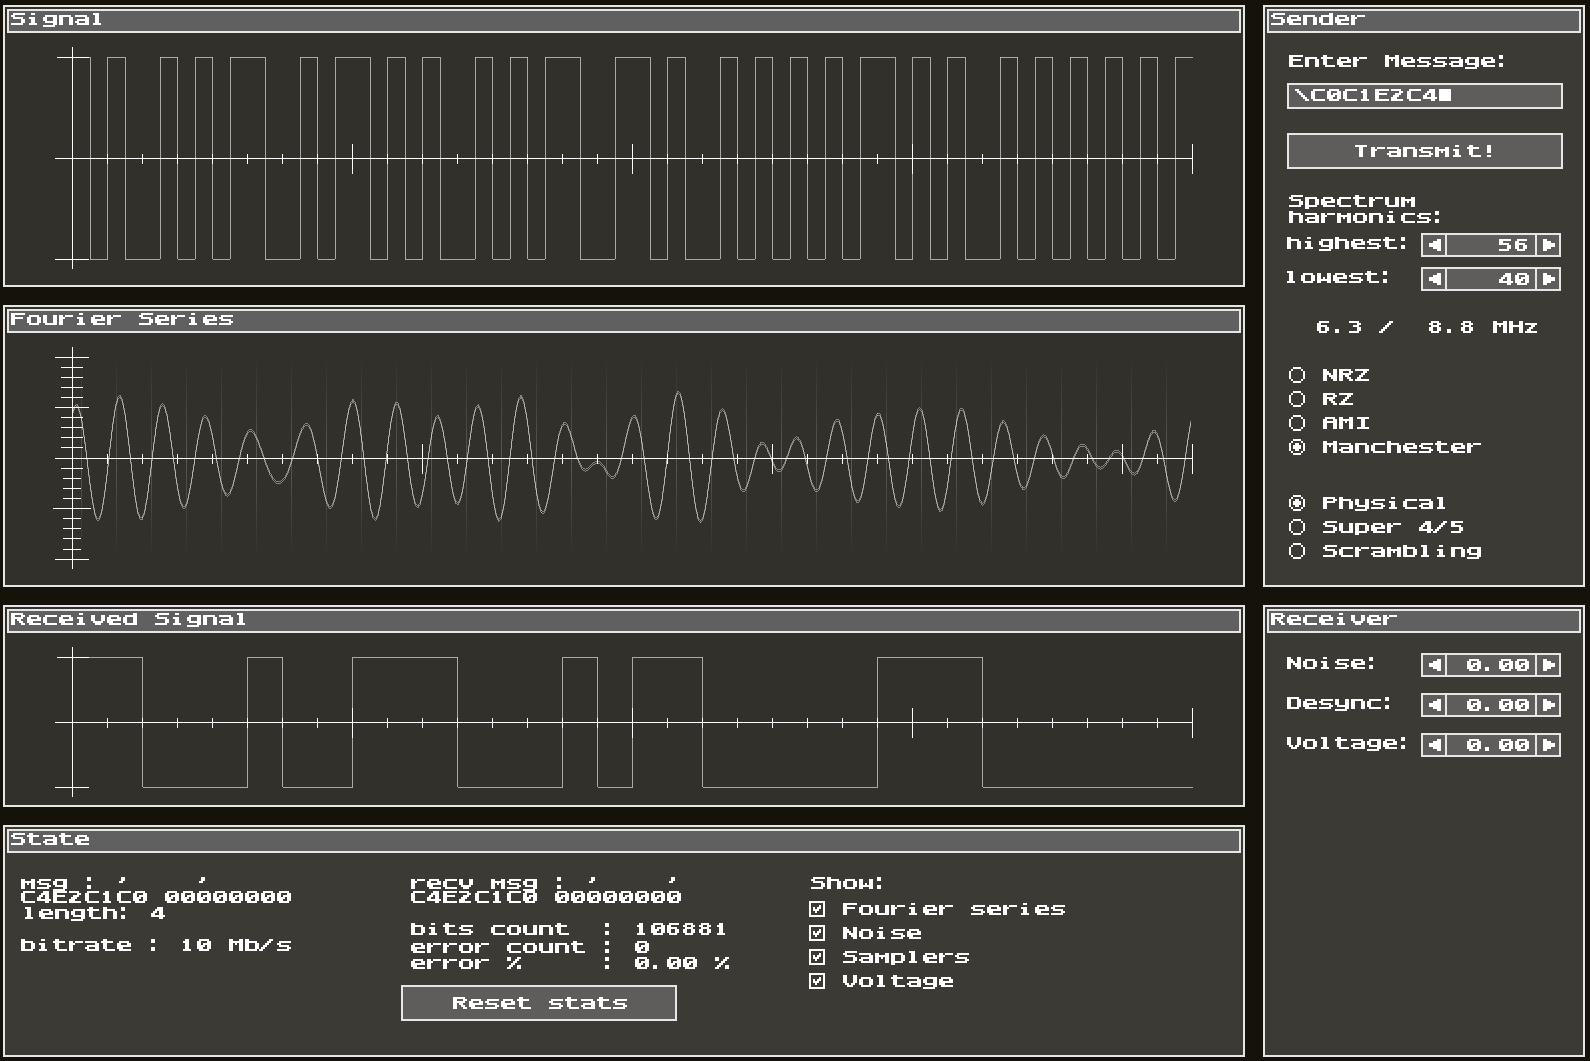
\includegraphics[width=0.95\linewidth]{./data/ideal_m2_min_f.png}
	\cutpic{0.2cm}{15cm}{./data/3_nrz45_voltage.png.jpg}
	\caption{Максимально допустимый уровень напряжения 0.02 для NRZ+4B/5B}
\end{figure}



% ------------------------------------------------


\subsection{NRZ + Scramble}

\subsubsection{Noise}

\vspace{-0.2cm}
\begin{wrapfigure}{r}{0.65\textwidth}
    \centering
    \cutpic{0.2cm}{11.5cm}{./data/3_nrzS_noise.png.jpg}
    \caption{Уровень шума 0.09 для NRZ + Scramble}
    \vspace{-5cm}
\end{wrapfigure}
\thispagestyle{empty}

Максимально допустимый уровень шума был определён с помощью программы \textit{Network Fourier} и составил \textbf{0.09}. Это граничное значение, при котором сигнал не искажается при воздействии произвольных гармоник.

\newpage

\subsubsection{Desync}

Максимально допустимый уровень рассинхронизации был определён с помощью программы \textit{Network Fourier} и составил \textbf{0.08}. Это граничное значение, при котором различие часов передатчика и приёмника не искажают сигнал.

\vspace{0.4cm}
\begin{figure}[h]
	\centering
	% 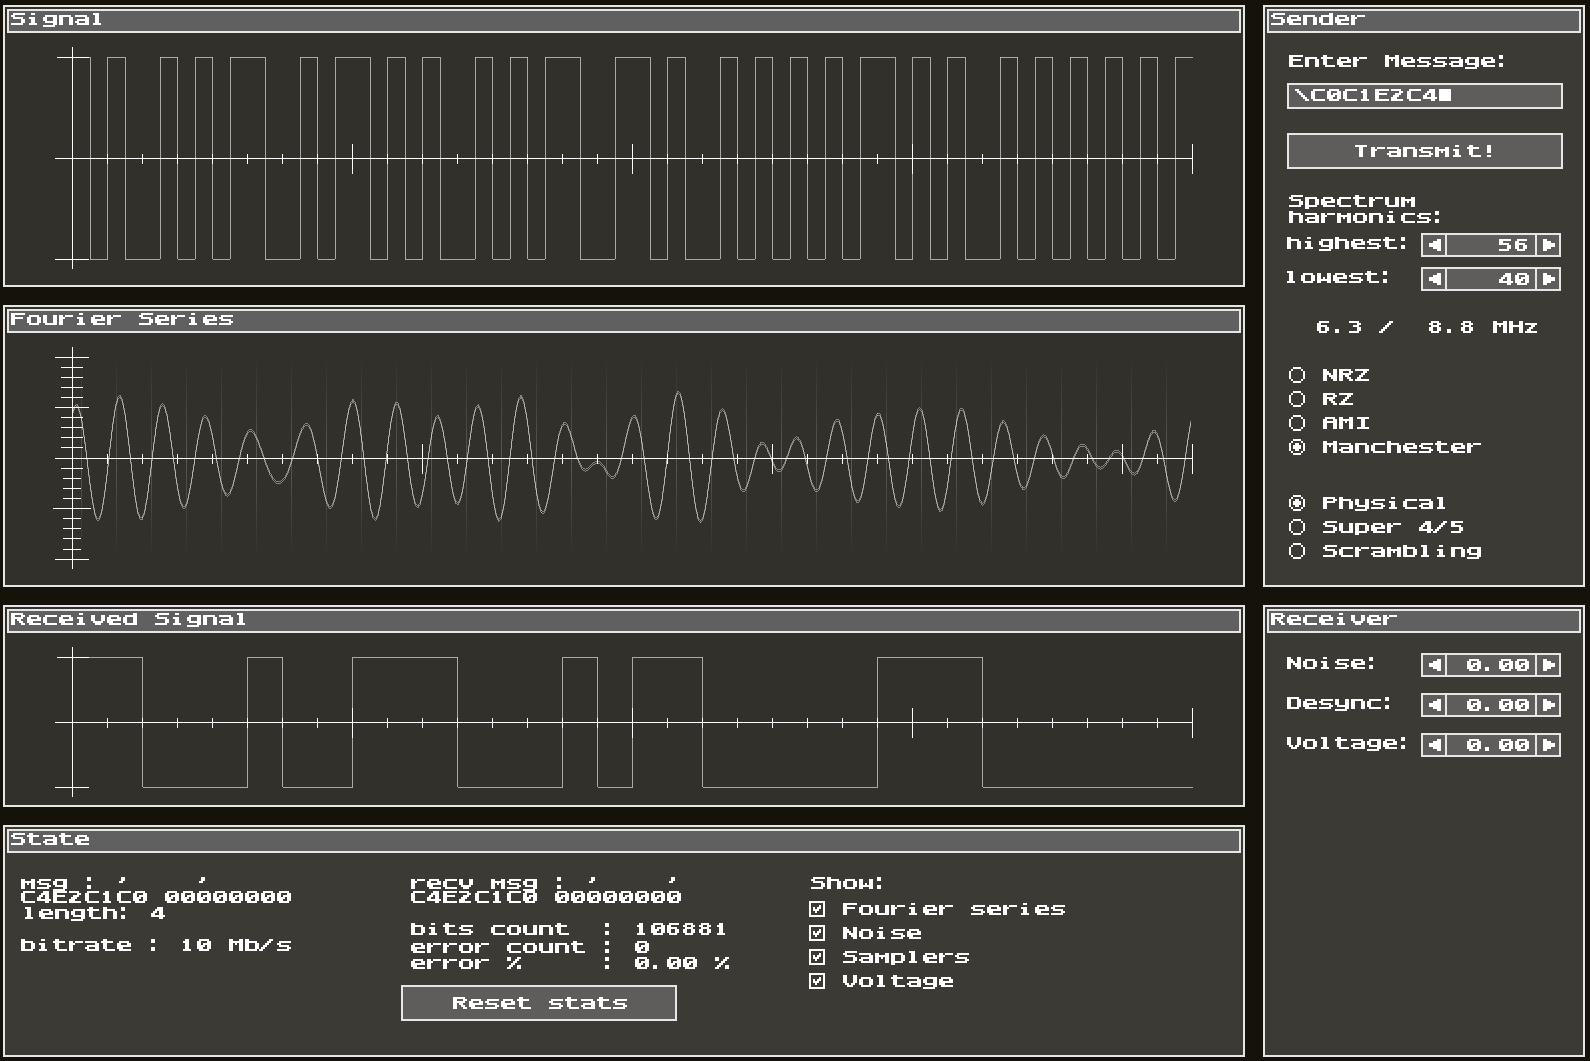
\includegraphics[width=0.95\linewidth]{./data/ideal_m2_min_f.png}
	\cutpic{0.2cm}{11.2cm}{./data/3_nrzS_desync.png.jpg}
	\caption{Макс. допустимый уровень рассинхрона 0.08 для NRZ+Scramble}
\end{figure}

\subsubsection{Voltage}

Максимально допустимый уровень напряжения был определён с помощью программы \textit{Network Fourier} и составил \textbf{0.37}. Это граничное значение, ниже которого мы не будем считывать сигнал.

\vspace{0.4cm}
\begin{figure}[h]
	\centering
	% 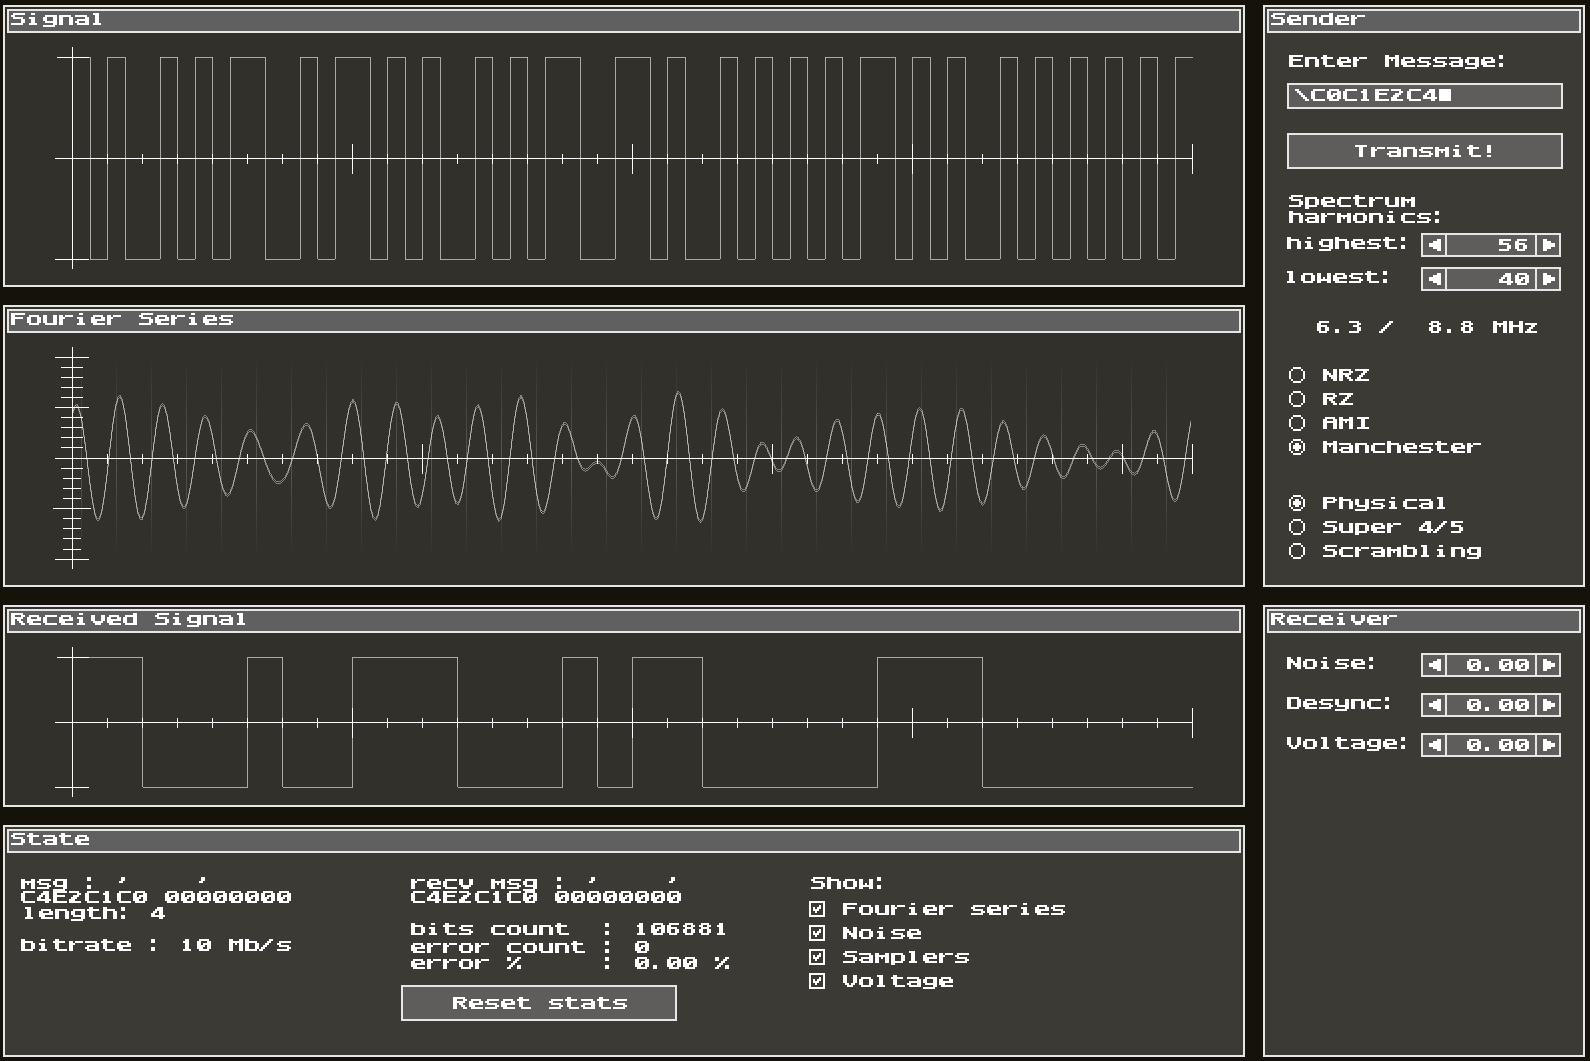
\includegraphics[width=0.95\linewidth]{./data/ideal_m2_min_f.png}
	\cutpic{0.2cm}{11.5cm}{./data/3_nrzS_voltage.png.jpg}
	\caption{Макс. допустимый уровень напряжения 0.37 для NRZ + Scramble}
\end{figure}


% ------------------------------------------------


\subsection{Выводы}

На данном этапе \underline{лучше остальных себя показали \textbf{NRZ} и \textbf{M2}}. 

У NRZ - лучшие показатели по уровню шума и рассинхронизации (0.2 и 0.35 соответственно), а уровень граничного шума (0.38) лучший после M2. Манчестер оказался невероятно устойчив к изменению уровня граничного напряжения до 1 В, что логично и объясняется тем, что он является импульсным кодом, и для его корректного приема неважен уровень напряжения, а важен переход напряжения от одного уровня к другому. Также, его уровень шума – на втором месте после NRZ (0.16), а уровень рассинхронизации (0.1) – на среднем уровне.

Худшие показатели у RZ (0.02, 0.02 и 0.16 при самой большой полосе пропускания). Этот метод показал себя хуже всех из-за необходимости обеспечения прочтения переходов сигнала в середине битового интервала в трех уровнях, что сложнее при ограниченной полосе пропускания, чем для двухуровневого M2, который также является импульсным.

NRZ+4B/5B и NRZ+Scramble показали результаты хуже чем сам NRZ. Такой результат обусловлен тем, что это потенциальные коды, и их плохая устойчивость к помехам обусловлена в том числе и содержанием сообщения, поэтому результаты по каждому из виду помех могут сильно отличаться друг от друга. Отметим только то, что NRZ+Scramble показал почти одинаковый уровень граничного напряжения (0.37) с NRZ (0.38), остальные параметры оказались хуже. А NRZ+4B/5B оказался хуже NRZ по всем параметрам.

